\section{Pianificazione}

	Per gestire lo sviluppo del progetto e soddisfare le scadenze riportate nella sottosezione \hyperref[riferimento_scadenze]{\S1.5}, il gruppo ha deciso di suddividere il periodo che va dalla sua formazione fino alla revisione di accettazione nelle seguenti quattro attività:
	\begin{itemize}
		\item Analisi dei requisiti
		\item Progettazione della \textit{technology baseline}
		\item Progettazione di dettaglio e codifica
		\item Validazione e collaudo
	\end{itemize}
	Ogni attività sarà poi suddivisa in più periodi, ad ognuno dei quali verrà associata una \glock{milestone}, riferita alla data di fine periodo, per il completamento delle singole attività previste al suo interno. In ogni singolo periodo sono, quindi, individuate più attività, le quali possono essere svolte sia sequenzialmente, sia con un certo grado di parallelismo, in base alle dipendenze che sussistono tra di loro.
	
	\subsection{Analisi dei requisiti}
	
		L'attività di analisi dei requisiti ha inizio il giorno 2019-11-15, successivamente alla formazione dei gruppi, ed è suddivisa in cinque periodi, con termine fissato per il giorno 2020-01-20, che precede la revisione dei requisiti del 2020-01-21.
		
		\subsubsection{Ruoli attivi}
		
			Durante questa attività è necessaria la presenza dei seguenti ruoli:
			\begin{itemize}
				\item responsabile;
				\item amministratore;
				\item analista;
				\item verificatore.
			\end{itemize}
		
		\subsubsection{Periodi}
		
			L'attività di analisi dei requisiti è stata suddivisa nei seguenti cinque periodi:
			
			\paragraph{Primo periodo (dal 2019-11-15 al 2019-12-06):}
			
				\begin{itemize}
					\item \textbf{Analisi dei capitolati:} studio individuale dei capitolati e discussione interna al gruppo dei pro e contro individuati da ogni componente, in modo da indirizzare l'interesse del gruppo su certi capitolati piuttosto che su altri;
					\item \textbf{Ricerca:} individuazione e studio degli strumenti e delle tecnologie di supporto da utilizzare per la gestione del progetto;
					\item \textbf{Normazione:} scelta delle regole da adottare durante lo sviluppo del progetto riguardanti la documentazione, la verifica e la gestione della configurazione;
					\item \textbf{Pianificazione delle attività:} decisione dell'organizzazione interna al gruppo riguardo i ruoli da assegnare ed i compiti da svolgere;
					\item \textbf{Studio di fattibilità:} impostato sulla base dell'analisi dei capitolati fatta in precedenza;
					\item \textbf{Analisi di qualità:} analisi preliminare riguardante le metriche da utilizzare per controllare e garantire la qualità del prodotto;
					\item \textbf{Verifica:} controllo della qualità di tutti i prodotti sviluppati durante il periodo attuale.
				\end{itemize}
			
			\paragraph{Secondo periodo (dal 2019-12-07 al 2019-12-16):}
			
				\begin{itemize}
					\item \textbf{Scelta del capitolato:} decisione definitiva riguardo il capitolato scelto;
					\item \textbf{Studio di fattibilità:} fine dello studio di fattibilità, basato al capitolato scelto;
					\item \textbf{Normazione:} scelta delle regole da adottare durante lo sviluppo del progetto riguardanti i processi primari e processi organizzativi;
					\item \textbf{Analisi di qualità:} analisi preliminare riguardante le metriche da utilizzare per controllare e garantire la qualità del prodotto;
					\item \textbf{Ricerca:} individuazione e studio degli strumenti e delle tecnologie implicate dal capitolato scelto, da utilizzare durante lo svolgimento del progetto;
					\item \textbf{Verifica:} controllo della qualità di tutti i prodotti sviluppati durante il periodo attuale.
				\end{itemize}
			
			\paragraph{Terzo periodo (dal 2019-12-17 al 2019-12-31):}
			
				\begin{itemize}
					\item \textbf{Normazione:} scelta delle regole da adottare durante lo sviluppo del progetto riguardanti i processi di supporto non ancora discussi;
					\item \textbf{Analisi dei casi d'uso:} analisi del prodotto e dei casi d'uso;
					\item \textbf{Pianificazione:} organizzazione interna al gruppo riguardo la pianificazione dell'intero progetto;
					\item \textbf{Analisi dei rischi:} individuazione dei rischi che possono presentarsi nello svolgimento del progetto;
					\item \textbf{Ricerca:} studio autonomo degli strumenti e le tecnologie da utilizzare per lo sviluppo del progetto;
					\item \textbf{Verifica:} controllo della qualità di tutti i prodotti sviluppati durante il periodo attuale.
				\end{itemize}
			
			\paragraph{Quarto periodo (dal 2020-01-01 al 2020-01-14):}
			
				\begin{itemize}
					\item \textbf{Analisi dei requisiti:} analisi dei requisiti e tracciamento;
					\item \textbf{Stesura della lettera di presentazione:} scrittura della lettera di presentazione con la quale ci si candida alla revisione dei requisiti;
					\item \textbf{Aggiornamento della pianificazione};
					\item \textbf{Aggiornamento della qualità};
					\item \textbf{Ricerca:} studio autonomo degli strumenti e le tecnologie da utilizzare per lo sviluppo del progetto;
					\item \textbf{Verifica:} controllo della qualità di tutti i prodotti sviluppati durante il periodo attuale.
				\end{itemize}
			
			\paragraph{Quinto periodo (dal 2020-01-15 al 2020-01-20):}
			
				\begin{itemize}
					\item \textbf{Preparazione presentazione:} redazione della presentazione da portare in sede di revisione e studio individuale.
				\end{itemize}


		\begin{landscape}

			\begin{figure}[H]
				\centering
				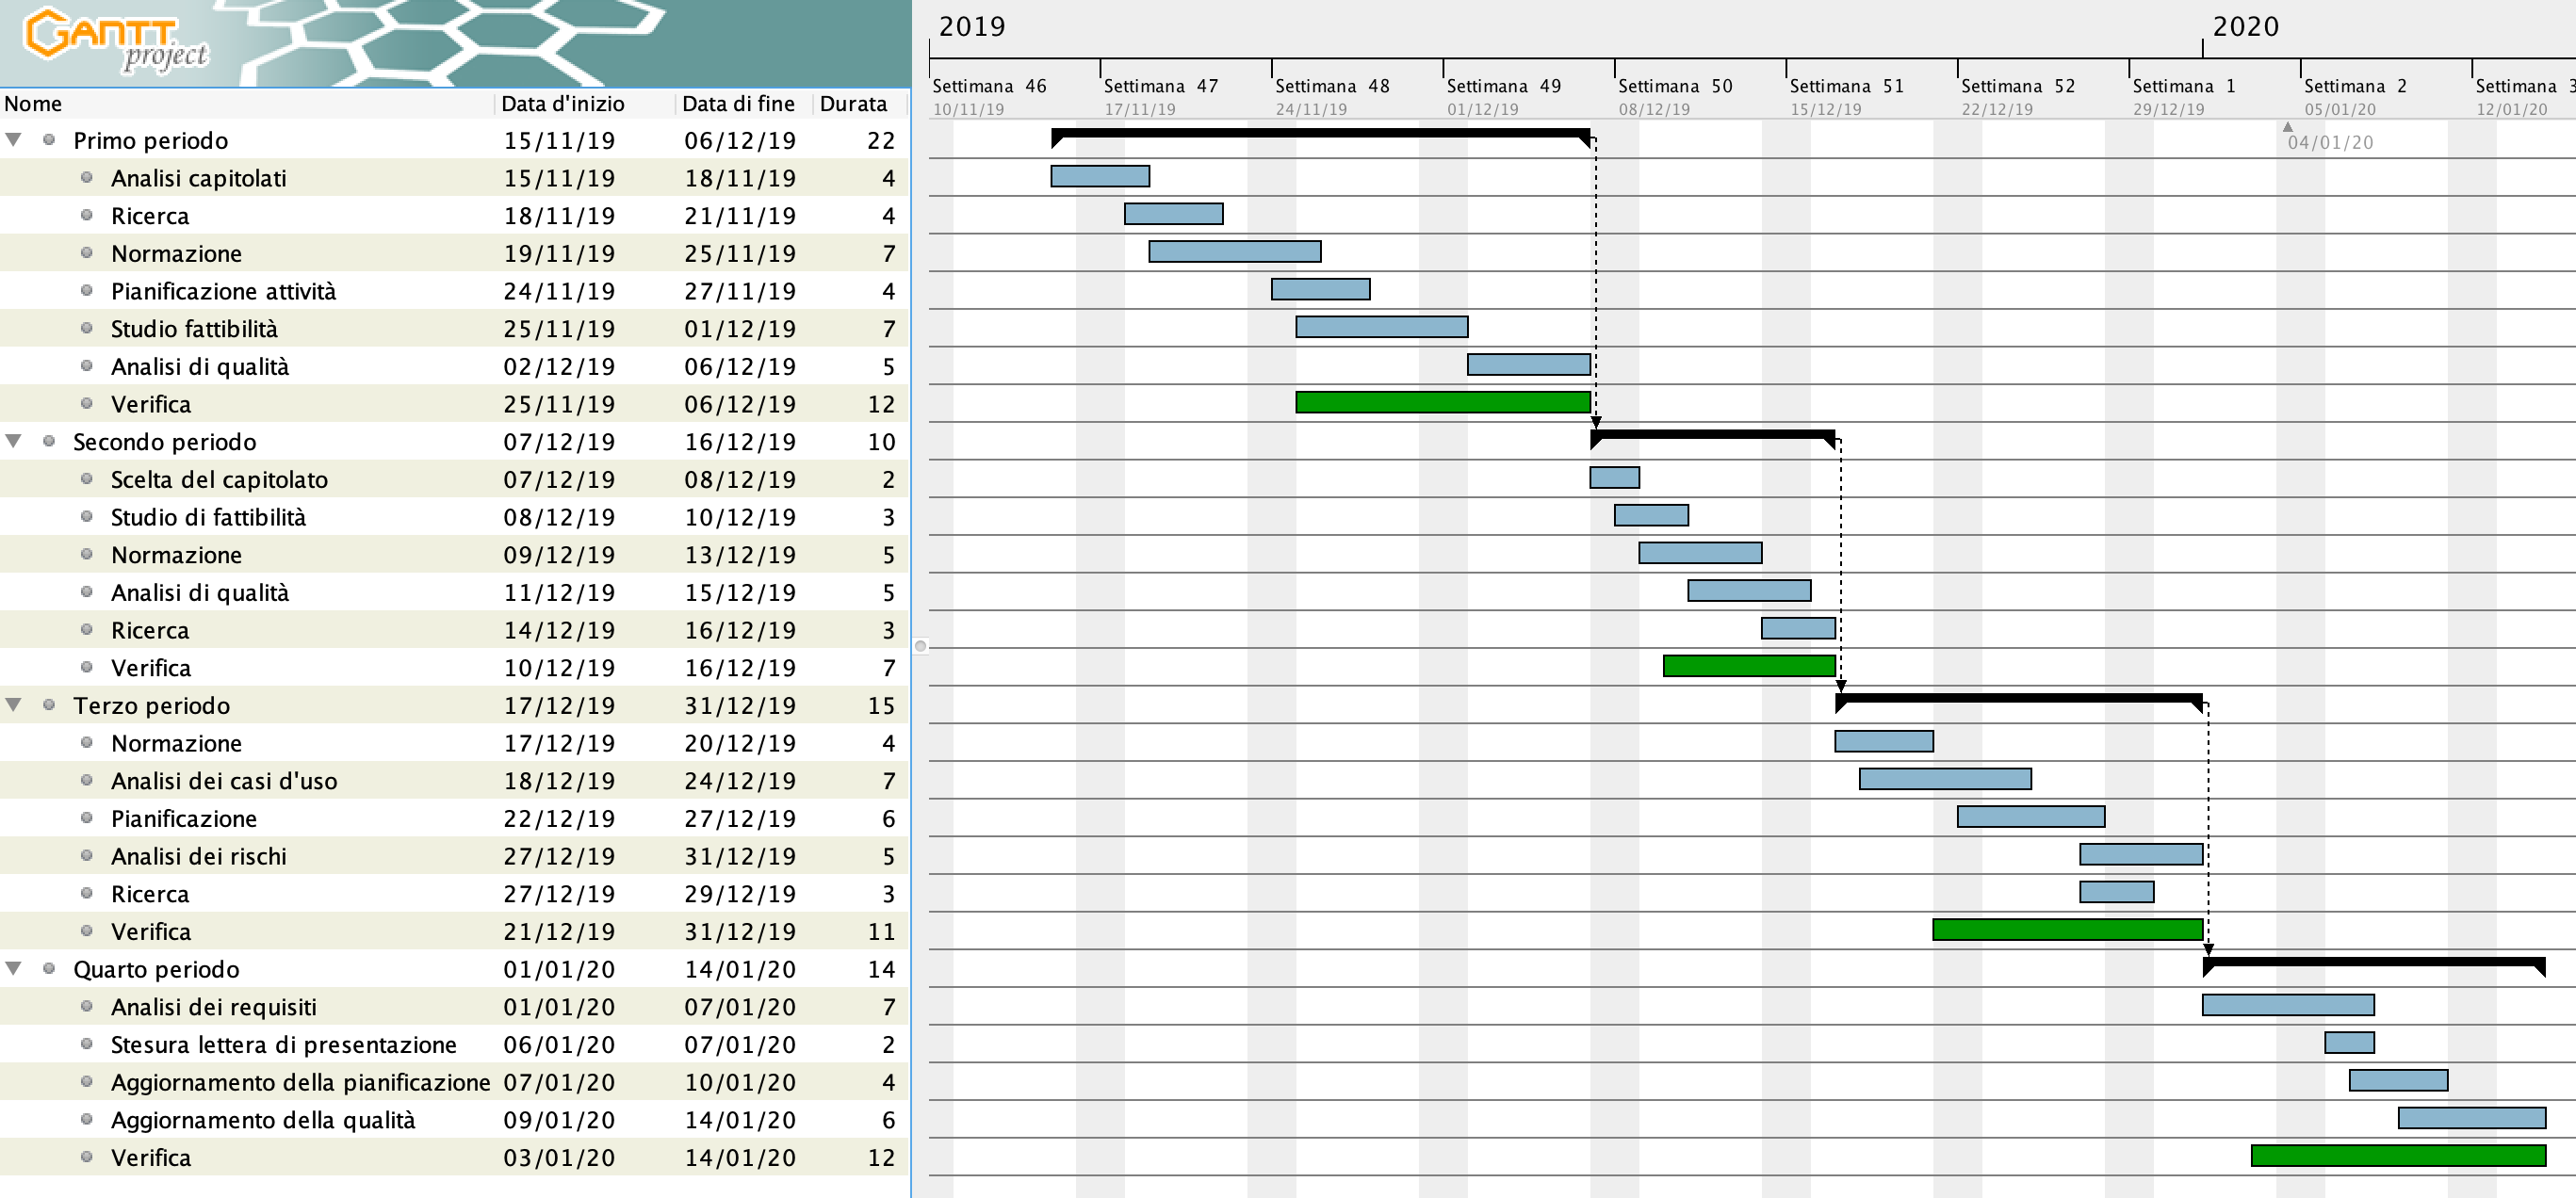
\includegraphics[width=\linewidth]{images/ganttAnalisi}
				\caption{Diagramma di Gantt dell'attività di Analisi dei Requisiti.}
			\end{figure}
				

		\end{landscape}

		\subsection{Progettazione della Technology Baseline}
	
			L'attività di progettazione della technology baseline ha inizio il giorno 2020-01-22, successivamente alla revisione dei requisiti, ed è suddivisa in tre periodi, con termine fissato per il giorno 2020-03-15, che precede la revisione dei requisiti del 2020-03-16.
			
			\subsubsection{Ruoli attivi}
			
				Durante questa attività è necessaria la presenza dei seguenti ruoli:
				\begin{itemize}
					\item responsabile;
					\item amministratore;
					\item analista;
					\item progettista;
					\item programmatore;
					\item verificatore.
				\end{itemize}
			
			\subsubsection{Periodi}
			
				L'attività di progettazione della technology baseline è stata suddivisa nei seguenti periodi:
				
				\paragraph{Primo periodo (dal 2020-01-22 al 2020-02-12):}
				
					\begin{itemize}
					 	\item \textbf{Normazione:} revisione ed eventuale aggiornamento delle norme;
					 	\item \textbf{Aggiornamento della pianificazione};
					 	\item \textbf{Aggiornamento della qualità};
					 	\item \textbf{Analisi dei requisiti:} revisione ed eventuale aggiornamento dei casi d'uso e dei requisiti, in base alle indicazioni ricevute;
					 	\item \textbf{Ricerca:} studio autonomo degli strumenti e le tecnologie da utilizzare per lo sviluppo del progetto;
					 	\item \textbf{Progettazione};
					 	\item \textbf{Verifica:} controllo della qualità di tutti i prodotti sviluppati durante il periodo attuale.
					\end{itemize} 	
				
				\paragraph{Secondo periodo (dal 2020-02-13 al 2020-03-08):}
				
					\begin{itemize}
						\item \textbf{Normazione:} aggiornamento delle norme;
						\item \textbf{Progettazione:} progettazione del \glock{proof of concept} che deve essere implementato;
						\item \textbf{Aggiornamento della pianificazione};
						\item \textbf{Codifica:} implementazione del \glock{proof of concept} progettato;
						\item \textbf{Stesura della lettera di presentazione:} scrittura della lettera di presentazione con la quale ci si candida alla revisione di progettazione;
						\item \textbf{Verifica:} controllo della qualità di tutti i prodotti sviluppati durante il periodo attuale.
					\end{itemize}
		
				\paragraph{Terzo periodo (dal 2020-03-09 al 2020-03-15):}
				
					\begin{itemize}
						\item \textbf{Preparazione presentazione:} redazione della presentazione da portare in sede di revisione e studio individuale.
					\end{itemize}

		\subsection{Progettazione di dettaglio e codifica}
			
			L'attività di progettazione di dettaglio e codifica ha inizio il giorno 2020-03-17, successivamente alla revisione di progettazione, ed è suddivisa in tre periodi, con termine fissato per il giorno 2020-04-19, che precede la revisione di qualifica del 2020-04-20.
			
			\subsubsection{Ruoli attivi}
			
				Durante questa attività è necessaria la presenza dei seguenti ruoli:
				\begin{itemize}
					\item responsabile;
					\item amministratore;
					\item progettista;
					\item programmatore;
					\item verificatore.
				\end{itemize}
			
			\subsubsection{Periodi}
			
				L'attività di progettazione di dettaglio e codifica è stata suddivisa nei seguenti periodi:
				
				\paragraph{Primo periodo (dal 2020-03-17 al 2020-03-27):}
				
					\begin{itemize}
						\item \textbf{Normazione:} revisione ed eventuale aggiornamento delle norme;
						\item \textbf{Aggiornamento della pianificazione};
						\item \textbf{Aggiornamento della qualità};
						\item \textbf{Progettazione:} miglioramento incrementale della progettazione fatta per il \glock{proof of concept};
						\item \textbf{Codifica:} implementazione prodotto software e test;
						\item \textbf{Scrittura manuale:} prima stesura;
						\item \textbf{Verifica:} controllo della qualità di tutti i prodotti sviluppati durante il periodo attuale.
					\end{itemize} 	
				
				\paragraph{Secondo periodo (dal 2020-03-28 al 2020-04-11):}
				
					\begin{itemize}
						\item \textbf{Normazione:} aggiornamento delle norme;
						\item \textbf{Aggiornamento della pianificazione};
						\item \textbf{Progettazione:} miglioramento incrementale della progettazione tramite \glock{design pattern};
						\item \textbf{Codifica:} primo rilascio;
						\item \textbf{Aggiornamento manuale};
						\item \textbf{Stesura della lettera di presentazione:} scrittura della lettera di presentazione con la quale ci si candida alla revisione di qualifica;
						\item \textbf{Verifica:} controllo della qualità di tutti i prodotti sviluppati durante il periodo attuale.
					\end{itemize}
		
				\paragraph{Terzo periodo (dal 2020-04-12 al 2020-04-19):}
				
					\begin{itemize}
						\item \textbf{Preparazione presentazione:} redazione della presentazione da portare in sede di revisione e studio individuale.
					\end{itemize}
		
		\subsection{Validazione e collaudo}	
		
			L'attività di validazione e collaudo ha inizio il giorno 2020-04-21, successivamente alla revisione di qualifica, ed è suddivisa in tre periodi, con termine fissato per il giorno 2020-05-17, che precede la revisione di accettazione del 2020-05-18.
			
			\subsubsection{Ruoli attivi}
			
			Durante questa attività è necessaria la presenza dei seguenti ruoli:
			\begin{itemize}
				\item responsabile;
				\item amministratore;
				\item progettista;
				\item programmatore;
				\item verificatore.
			\end{itemize}
			
			\subsubsection{Periodi}
			
				L'attività di validazione e collaudo è stata suddivisa nei seguenti periodi:
		
				\paragraph{Primo periodo (dal 2020-04-21 al 2020-05-1):}
			
					\begin{itemize}
						\item \textbf{Normazione:} revisione ed eventuale aggiornamento delle norme;
						\item \textbf{Aggiornamento della pianificazione};
						\item \textbf{Aggiornamento della qualità};
						\item \textbf{Completamento progettazione};
						\item \textbf{Verifica:} controllo della qualità di tutti i prodotti sviluppati durante il periodo attuale.
					\end{itemize} 	
				
				\paragraph{Secondo periodo (dal 2020-04-02 al 2020-05-10):}
				
					\begin{itemize}
						\item \textbf{Codifica:} rilascio ultima versione;
						\item \textbf{Completamento manuale};
						\item \textbf{Verifica:} controllo della qualità di tutti i prodotti sviluppati durante il periodo attuale, in particolare sono eseguiti i test per la verifica del software.
					\end{itemize}
		
				\paragraph{Terzo periodo (dal 2020-05-11 al 2020-05-17):}
				
					\begin{itemize}
						\item \textbf{Preparazione presentazione:} redazione della presentazione da portare in sede di revisione e studio individuale.
					\end{itemize}
	
